%%% DOCUMENT SETUP %%%
\documentclass[11pt,a4paper,onecolumn]{article}
\usepackage[english]{babel}

%%% LAYOUT %%%
\usepackage{fullpage}
\usepackage[a4paper]{geometry}
\usepackage[parfill]{parskip}
\usepackage{multicol}
\usepackage{footnote}

%%% GRAPHICS %%%
\usepackage{graphicx}
\usepackage{color}
\usepackage{graphics}
\usepackage{rotating}
\usepackage{subfig}
\usepackage{amsmath}
\usepackage{amssymb}
\usepackage{amscd}
\usepackage{xfrac}
\usepackage{float}
\usepackage{dsfont}

%%% FONT %%%
\usepackage{ifxetex}
\ifxetex
  \usepackage{fontspec}
    \setmainfont{Linux Libertine O}
  \usepackage{xunicode}
  \usepackage{microtype}
\else
  \usepackage[T1]{fontenc}
  \usepackage[latin1]{inputenc}
  \usepackage{times}
  \usepackage{microtype}
\fi

%%% Coding %%%
\usepackage{listings}
\usepackage{pseudocode}

%%% TITLE PAGE %%%
\author{Jeroen Hofman  \\
[15pt] University of Amsterdam (\textsc{UvA})}

\title{Concurrent Programming week 1:\\
  Performance of sequential code.
		}

\begin{document}
\maketitle
\captionsetup{width=0.8\textwidth}
\lstset{language=Python,breaklines=true,backgroundcolor=\color{white},frame=single}
\thispagestyle{empty}

%%% ABSTRACT %%%
\begin{center}
\begin{abstract}
\small{In this report we look at a piece of sequential code describing heat diffusion on a cylindrical surface. After machine benchmarking and compiler optimization we looked at scaling between problem size and execution time for fixed rows and columns respectively. The difference found in total execution time is caused by mixed boundary conditions in the problem, whereas there is no difference in execution time per iteration. Furthermore we found a significant decrease in performance around a matrix size of 460x460, indicating a cache size of 4MB.} \\
\end{abstract}
\end{center}

%%% TABLE OF CONTENTS %%%
\newpage
\tableofcontents
\newpage

\section{Experimental setup}
In this section we first describe the benchmarks of the machine, more precisely the specifics of the parallel hardware and an estimate of the FLOP/s. Secondly we look at the structure of the sequential code implemented to model a simple heat diffusion model. Thirdly we optimize the compiler for the specific model at hand.

\subsection{Machine benchmarking}
Since we ultimately want to measure the performance of the sequential code that is written, we want to obtain an estimate of the FLOP/s for the machine one which the code is executed. This is done by implementing a simple program, provided by the instructors of the course, performing five different floating point operations during a time span of fifteen seconds. The operations should converge to $\pi$. The program was tested on two machines:

\begin{itemize}
\item 
  HP Pavilion dm1 - OS: Ubuntu 11.10, Kernel: Linux 3.0.0-14-generic, Memory: 4 GB, Processor: AMD E-350 dual core.
\item
  LISA - for specifications see \cite{LISA}, we will use the 8-core nodes with 24GB memory.
\end{itemize}

The code is executed three times per machine and the minimum is reported in Table \ref{tab:benchmark} below:

\begin{table}[H]
  \centering
  \begin{tabular}{l | c | r}
    Machine & FLOP/s & Approximation of $\pi$ \\
    \hline
    HP Pavilion dm1 & 196170013 & 3.141592655288159 \\
    & 196268141 & 3.141592651890593 \\
    & 195838531 & 3.141592655291024 \\ 
    LISA & 615233452 & 3.141592654482680 \\
    & 615377252 & 3.141592654129703 \\ 
    & 615350123 & 3.141592654129727 \\
  \end{tabular}
  \caption{Results for the benchmark code.}
  \label{tab:benchmark}
\end{table}

Clearly the node (an 8-node with 24GB memory) is much faster than the laptop ($6.15 \; 10^8$ versus $1.96 \; 10^8$), which is expected since the LISA node is equipped with a quad-core while the laptop only has a dual-core processor. LISA also approximates $\pi$ better from the 9th decimal on (the 9th decimal should be a 3). 

\subsection{Structure of the sequential code}
\label{sec:struc}

The problem that needs to be solved by the sequential code is a heat diffusion problem on a cylinder in two dimensions. Given an arbitrary matrix size and a given temperature and conductivity value defined for each point on the grid, we want to compute the temperature of the system after a certain time, calculated in terms of iterations. The temperature of a grid point in iteration $i+1$ depends on the temperature of the grid point at iteration $i$ and the temperature of the surrounding neighbors (8 in the case of a two-dimensional grid), where the relative weights are given by the conductivity $c$ and $1-c$ for the grid point and its neighbors respectively. The joint value of the neighbors is calculated by taking the weighted average of the four direct neighbors (top, bottom, left, right) with weight $\sfrac{\sqrt{2}}{\sqrt{2}+1}$ and the weighted average of the four diagonal neighbors with weight $\sfrac{1}{\sqrt{2}+1}$.

In our simulation this boils down to defining two arrays, one with the current temperatures and another one with the new temperatures calculated in the iteration step by the method above. The top and bottom boundaries of the grid are fixed, we have implemented a halo (extra) row at the top and bottom boundaries which has the values of the top and bottom row of the initial values of the initial (given) temperature matrix. These halo values do not change during the calculation. Similarly to mimic the continuous boundary conditions we add two halo columns on the left and right of the matrix, where the left column has the same values as the right column of the original (given) matrix, and the right column has the same values as the left column of the original (given) matrix. This copying is performed every iteration step. The advantage is that with this extra frame around the matrix it is easy to calculate the new temperature matrix, the same algorithm applies for all points in the original matrix (so no modulo operators and if-else statements and the like).

Every iteration step we calculate a new temperature matrix and also calculate the maximum of the point wise difference between the old and new temperature matrix. The simulation ends either after this difference reaches some minimum value (the threshold), or the maximum number of iterations is reached. Periodically during the simulation and at the end of the simulation we report the average temperature, the minimum/maximum temperature and the execution time of the code so far. This execution time is used to calculate the FLOP/s of the code. The calculation is such that they are supposed to be 12 FLOPs in every iteration, however in our code the number of FLOPs is 13. For correcting and checking purposes of the code the calculation of the FLOP/s is not altered, however the results of the FLOP/s given by the output of the code are multiplied by 13/12 and given as such in the rest of this report. The original value is given in parentheses behind this better approximation. It is important to note that this factor is only accurate if the reporting frequency of intermediate results is low. In all the results and output given in the rest of the report there were no intermediate results printed, only the final output, so that our conversion is a good approximation.

\subsection{Technical details of the code}
Here follow some technical details of the code as implemented in compute.c. Where appropriate we state the line number of the specific piece of code discussed.

The two temperature arrays in the code are two-dimensional, however they are allocated as one-dimensional arrays but can be called in two-dimensional form (lines 27, 33). The two arrays are called currIt and nextIt. First we initialize currIt by filling it with some input temperature matrix. Note that currIt and nextIt are larger than this input matrix, to have space available for the extra frame as described above. The extra row at the top and bottom of currIt are filled as well by the values of the row beneath and above it respectively (lines 53 - 70). Note the nextIt is also filled already with these two rows, as they are static during the whole computation. Before we start the main iteration loop we initialize the time structs which will measure the time in microseconds (line 76 - 78).

Every iteration we first copy the second column to the last column and the previous to last column to the first column in currIt to implement the continuous boundary conditions. We then proceed with the heart of the code, which is the calculation of the new temperature grid. For every grid point we first read the conductivity value at that point, and then proceed with calculating a temperature value for that grid point for nextIt, given the temperature value in currIt (line 102 - 120). Note that the neighbor weights are constants and hence hard-coded. After finishing this loop we simply swap the pointers of the arrays (line 122 - 126), which is effectively the same as copying nextIt to currIt for the next iteration, but much faster. After this swapping we either compute the maximum point wise difference or we do a more thorough evaluation for an intermediate reporting of the results. This intermediate reporting also causes an extra FLOP for the computation of the average. The minimum, maximum and difference of the temperatures are calculated with fmin and fmax, which are fast math.h routines for floating point comparisons. At the end of the loop the maximum point wise difference is compared with the threshold and the loop ends if this difference is smaller than the threshold (line 176 - 182). After the loop another final report round is calculated. Note that if the last intermediate report coincides with the end of the iteration, it will report twice but with different values, since it first calculates all the values for the report session in the loop and gives a execution time, and then it proceeds with again calculating all the values, which will be the same, except of course for the execution time. However intermediate reporting is not used in this report, other than for debugging the code.

One last remark is the use of the restrict data type. The two temperature arrays as well as an extra variable for the swapping of the arrays are of type \textbf{double *restrict} where the restrict type gives faster compilation since the compiler assumes the pointers do not point to the same locations during their lifetime. While this is not strictly true in the code since they are swapped, during the swapping there are no operations performed with the objects associated with the pointer and hence the restrict type can still be used, giving a significant speedup of the code (around 20\%).

\subsection{Compiler optimization}
We optimize the compiler by looking at different options as given in Table \ref{tab:compiler} below. Each program with specific compiler options was executed three times on the LISA cluster (8 cores, 24GB memory) with GCC version 4.4.5 and the minimum is reported here. We used N = 500, M = 500, a threshold value of 0 and a maximum number of iterations of 3000. 

\begin{table}[H]
  \centering
  \begin{tabular}{l | c | r}
    Compiler option & Execution time & FLOP/s \\
    \hline
    -O2 & 15.97 & 6.11 (5.64) $10^8$\\
    -O3 & 16.36 & 5.95 (5.50) $10^8$\\
    -Os & 16.37 & 5.93 (5.47) $10^8$\\
    -O2 -march=native & 15.97 & 6.10 (5.63) 10$^8$ \\
    -O2 -ffast-math & 16.03 & 6.08 (5.61) 10$^8$ \\
    -O2 -fomit-frame-pointer & 16.05 & 6.08 (5.61) $10^8$ \\
    -O2 -fprofile-use & 6.91 & 1.41 (1.30) $10^9$ \\
    \end{tabular}
  \caption{Compiler option results}
  \label{tab:compiler}
\end{table}

Based on the results above, for this specific problem the -O2 parameter seems to give the best overall performance. The parameter -fprofile-use gives a significant speed-up of the code, by first running -fprofile-generate and then using -fprofile-use in subsequent compilations of the code. Based on the above table we use -O2 and -fprofile-use as the 'base'  parameters. Although the above table suggests that the other parameters (-march=native, -ffast-math and -fomit-frame-pointer) do not contribute much to a speedup of the code execution, they do contribute when used together with the -fprofile-use parameter. The use of the parameters -O2 -fprofile-use -march=native -ffast-math -fomit-frame-pointer gives an execution time of 4.78 seconds, with an estimated FLOP/s of $1.88 \; (2.04) \; 10^9$. The execution times for combinations of -O3 and -Os with -fprofile-use were also measured, but these parameter settings performed worse than -O2 with -fprofile-use.

A downside of the use of -fprofile-use is that the code has to be compiled and run once with -fprofile-generate, which takes more time. However, if one plans to execute the code multiple times after wards (as in the following experiments), it is definitely worth wile in terms of time. 

From now on in this report we will use the above mentioned combination of optimal compiler configuration and we will run all experiments on a node of LISA with 8 cores and 24GB memory.

\section{Results}
All results in this section are generated by a LISA node with 8 cores and 24GB memory. The input files for the temperature are gradientxxx\_xxx.pgm and for the conductivity pat1xxx\_xxx.pgm. If not specified the default values are used (for instance for the lowest and highest initial temperature).

\subsection{Scaling}
We run the sequential code for heat diffusion as described in Section \ref{sec:struc} first without a maximum number of iterations. We set the threshold to $10^{-9}$ and we compute first for fixed N and M = $\{50,200,1000\}$ the execution time and the FLOP/s. Then we repeat the experiment but we fix M and set N = $\{50,200,1000\}$. We repeat every experiment three times, the minimum of the execution times (and hence the maximum FLOP/s) are given in Table \ref{tab:scaling} below.

\begin{table}[H]
  \centering
  \begin{tabular}{l | c | c | c | c | c}
    Row/column size & \# Iterations & Max. difference & Avg. temperature & Execution time & FLOP/s \\
    \hline
    \multicolumn{6}{c}{Fixed N = 100 } \\
    \hline
    M = 50 & 63143 & 9.998977 $10^{-6}$ & -4.283618 $10^{-5}$ & 2.368444 & 1.73 (1.60) $10^9$\\
    M = 200 & 104694 &  9.999004 $10^{-9}$ & -1.953911 $10^{-5}$ & 15.60905 & 1.74 (1.61) $10^9$\\
    M = 1000 & 430369 & 9.999802 $10^{-9}$ & -2.859329 $10^{-5}$ & 312.3580 & 1.79 (1.65) $10^9$\\
    \hline
    \multicolumn{6}{c}{Fixed M = 100 } \\
    \hline
    N = 50 & 27434 & 9.997348 $10^{-9}$ & 8.328201 $10^{-6}$ & 1.006071 & 1.78 (1.64) $10^9$\\
    N = 200 & 238890 & 9.999706 $10^{-9}$ & -1.721664 $10^{-4}$ & 35.73031 & 1.73 (1.60) $10^9$\\
    N = 1000 & 4131628 & 9.999999 $10^{-9}$ & -7.96583 $10^{-3}$ & 3079.855 & 1.74 (1.61) $10^9$\\
  \end{tabular}
  \caption{Results for fixed N (top) and fixed M (bottom)}
  \label{tab:scaling}
\end{table}

To estimate the scaling of the execution time with the problem size we can make a simple quadratic fit through the three data points obtained for a fixed N and M respectively. The result is shown in figure \ref{fig:scaling} below. From the figure we obtain the following scaling parameters: 2.97 $10^{-8}$ for fixed N and 3.76 $10^{-7}$ for fixed M (the factor in front of $x^2$ in the fits). The scaling parameter for fixed M is much higher than for fixed N. By looking at the code the only difference which exists between number of rows and number of columns is the copying of two columns every time step to produce the halo columns. This copying is not affected when N is fixed, but it is affected when the number of columns of fixed (and hence the number of rows is not). However, if this would be the cause of this discrepancy in scaling parameters the FLOP/s would be affected as well since this copy operation is not included in the FLOP count. There is however not a significant difference between FLOP/s, as shown in Table \ref{tab:scaling}.

\begin{figure}[H]
  \centering
  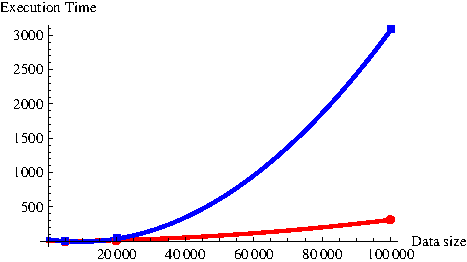
\includegraphics[width=0.7\textwidth]{scaling.pdf}
  \caption{The data size versus the total execution time for fixed N (red) and fixed M (blue) obtained from Table \ref{tab:scaling}.}
  \label{fig:scaling}
\end{figure}

Actually there is a much simpler reason that these scaling parameters are different, which has to do with both the temperature profile (in this case the temperature profile is a gradient and the conductivity profile pat1) and with the dynamics caused by the cylindrical form. If we divide the execution time by the number of iterations and obtain a scaling parameter in this way by fitting to the data, we find a scaling parameter (in the linear term) of 7.50 $10^{-9}$ for fixed N and 7.55 $10^{-9}$ for fixed M, which is nearly the same. So the execution time per iteration is the same for both fixed N and fixed M and grows linearly, as we would expect judging from the code. 

The reason that the total execution time as seen in Figure \ref{fig:scaling} is different for fixed N and fixed M respectively and grows quadratically, is caused by a different stretching of the temperature profile and hence a different iteration number for which the calculation reaches the threshold. It is more importantly caused by the fact that adding a column adds only a static boundary condition while adding a row adds a continuous boundary condition. Adding an extra static boundary point will cause the system to reach lower point wise maximum difference values faster than adding a continuous boundary point because the system will fluctuate more in the latter case. Consider for instance a situation with many columns but very few rows. Points in the grid will reach equilibrium very fast because they are being 'fed' values from the static boundaries. If on the contrary we have a situation with many rows but few columns, the influence of this static boundary is small and points somewhat in the middle of the system will initially fluctuate with the values around them, rather than adjusting to the static boundary values right away. 

\begin{figure}[H]
  \centering
  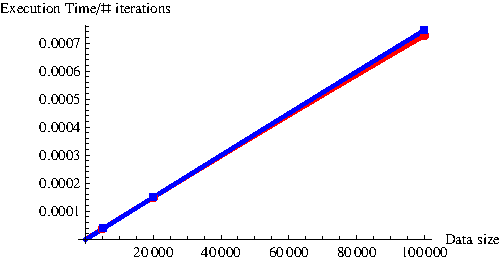
\includegraphics[width=0.7\textwidth]{scalingf.pdf}
  \caption{The data size versus the execution time per iteration for fixed N (red) and fixed M (blue) obtained from Table \ref{tab:scaling}.}
  \label{fig:scaling}
\end{figure}

\subsection{Cache size}
If we compare the FLOP/s for two different flop sizes, namely N = M = 25 and N = M = 3000, we obtain (again taken the minimum over 3 runs, threshold is 0):

\begin{table}[H]
  \centering
  \begin{tabular}{l | c | c | c | c | c}
    Problem size & \# Iterations & Max. difference & Avg. temperature & Execution time & FLOP/s \\
    \hline
    N = M = 25 & 1000000 & 0.0 & 1.220722 $10^{-4}$ & 3.740644 & 2.01 $10^9$ \\
    N = M = 3000 & 1000 & 1.418835 $10^{-2}$ & 2.343403 $10^{-2}$ & 1.032930 $10^2$ & 1.05 $10^9$
  \end{tabular}
\end{table}

From the above it is seen that the FLOP/s drops by nearly 50\% with increasing the system size from 25 to 3000. Below in Figure \ref{fig:cache} there are some more results shown for the FLOP/s as a function of system size.

\begin{figure}[H]
  \centering
  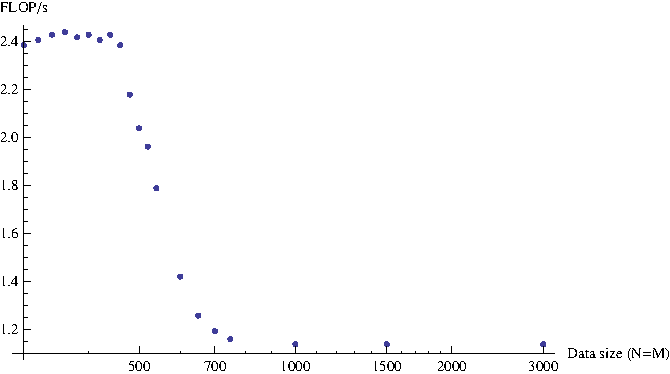
\includegraphics[width=0.7\textwidth]{cache.pdf}
  \caption{System size (N=M) against the measured FLOP/s.}
  \label{fig:cache}
\end{figure}

The figure shows that there is a significant drop in FLOP/s around a matrix size of 460. If we assume the data for the program is stored in the cache, and we furthermore assume that the large chunk of data is made up of the two temperature arrays, we find a cache use of $460² * 8 * 2 \approx 3.39$MB which would imply a cache size of about 4MB. The system used on LISA is a processor with 8MB cache size (Intel XEON L5520 \cite{LISA}), but hyper-threading is enabled on all processors. It is not easy to find relevant information on the implementation of hyper-threading on the nodes used on LISA, but the results above suggest that each (hardware) thread is allowed 4MB of cache since there are two hardware threads running per core.

\section{Conclusions}

We investigated the performance of a piece of sequential code describing heat diffusion on a two-dimensional cylinder. After compiler optimization and machine benchmarking we looked at scaling factors where we varied the column size (keeping the row size fixed) and the row size (keeping the column fixed). The total execution time scales differently (with fixed threshold) for both cases mainly because the adding of an extra row is inherently different from adding an extra column, due to different boundary conditions. The execution time per iteration is nearly the same for both cases, implying there is no difference in the way columns and rows are treated from a strict encoding perspective.

Furthermore we looked at performance for increasing problem size and found a significant change around a matrix size of 460 (keeping row and columns equal). This implies a cache size of our system around 4MB instead of the 8MB given by system specifications, this could be explained by the hyper-threading functionality of the core.


%%% BIBLIOGRAPHY %%%
\begin{thebibliography}{7}
\bibitem{LISA}
  http://sara.nl/systems/lisa/description
\end{thebibliography}

\end{document}
